

%Tähän voisi laittaa kuvan komponenttien asemmoitumisesta toisiinsa.
\subsubsection{Asiakaslaite}
Asiakaslaite (user equipment) on yleisnimitys laitteelle, joka on reunan tai pilven tarjoamien palveluiden asiakas. 
Asiakaslaitteen tyyppiä ei ole rajattu ja asiakaslaite voi olla esimerkiksi älypuhelin, älylasit tai vaikka verkkoyhteydellä varustettu auto. 
Yhdistävänä tekijänä on siis jonkinlainen yhteys reuna- tai pilvipalveluihin. Yleisesti yhteys on tyypiltään langaton. 
Tässä tutkielmassa asiakaslaitteella tarkoitetaan älypuhelinta, jollei toisin mainita.

Verkkohierarkian näkökulmasta asiakaslaitteet ovat lehtisolmuja. Tämä tarkoittaa että asiakaslaitteet toimivat ainoastaan palveluiden kuluttajina eivätkä siis tarjoa itse palveluita. Myöskään kulutettavien palveluiden tyypillä ei ole juurikaan merkitystä, kun asiaa käsitellään infrastruktuuri/arkkitehtuuritasolla.

Esimerkkinä asiakaslaitteen toiminnasta reunapalvelua hyödyntäen voisi olla ajoneuvo, joka käyttää reunapalveluita tiedon välittämiseen muille lähistöllä oleville ajoneuvoille.


%Asiakaslaite on yleisnimitys laitteelle, joka hyödyntää reunan tai pilven tarjoamia palveluita jonkin tietoliikenneyhteyden avulla.
%Reunalaskentaa käsittelevässä kirjallisuudessa asikaslaitteeseen viitataan usein UE (User Equipment) termillä. 
%Se mitä konkreettista laitetta asiakaslaitteella tarkoitetaan riippuu kontekstista. 
%Tässä tutkielmassa asiakaslaitteella tarkoitetaan älypuhelinta jollei toisin mainita. 
%Esimerkkinä jostain toisesta asiakaslaitteesta on auto, joka on varustettu mobiiliverkkoyhteydellä. Auto voi käyttää reunapalveluita esimerkiksi kommunikoidakseen muiden lähistöllä olevien autojen kanssa.
%Asiakaslaitteet verkkoyhteyksien muodostaman hierarkian "lehtisolmuja" joka tarkoittaa että ne eivät enää tarjoa palveluitaan muille asiakaslaitteille. 


\subsubsection{Reuna} \label{reunatoimijat}
Reuna koostuu useista toiminnallisista entiteeteistä, jotka voidaan jakaa sekä fyysisiin, että loogiisin entiteetteihin. On kuitenkin hyvä ymmärtää koko reunan käsittävä reuna-alue, joka esitellään ensimmäisenä. Tämän jälkeen esitellään reunasolmu, joka on reunajärjestelmän keskeisin fyysinen rakennuspalanen. Lopuksi esitellään pääasiassa ohjelmallisen tason toimivat toimijat reuna-alusta ja reunasovellus.

\paragraph{Reuna-alue} 
Reuna-alue tai reuna ei ole mikään tarkasti rajattu alue, vaan reunalla usein tarkoitetaan jonkin tietyn kontekstin mukaista reunaa. 
Yleisesti reunalla voidaan viitataan alueeseen, joka ulottuu asiakaslaitteelta runkoverkkoon asti. Reunalle ei siis ole tarkkaa määritelmää.
Reuna-alue rajautuu siinä esiintyvien toimijoiden mukaan jollekkin välille. 
Esimerkiksi mobiiliverkon tukiasemien yhteyteen rakennettua reunajärjestelmää käsiteltäessä, reunalla tarkoitetaan ainoastaan reunajärjestelmän asiakaslaitteita palvelevien osien muodostamaa vyöhykettä. 
Yleisenä nyrkkisääntönä voidaan pitää verkkoyhteyksien viivettä, suhteessa muuhun internettiin, koska reuna-alueella viiveiden tulisi siis olla muuta internettiä nopeampia. Toisin sanoen palveluiden tulisi sijaita lähempänä.


\paragraph{Reunasolmu} 
Tämän tutkielman kontekstissa reunasolmulla (mobile edge host) tarkoitetaan yksittäistä reunalaskentaa suorittavaa entiteettiä. Reunasolmu voi koostua esimerkiksi mobiilitukiaseman ja palvelinlaitteiston muodostamasta kokonaisuudesta. Reunasolmu sisältää vähintään reunasovelluksien suorittamiseen tarvittavan laitteiston, sekä toiminnallisesti reunasovelluksien suorittamiseen tarvittavat hallinnolliset toimet. 
Kuten aiemmin mainittu, reunajärjestelmä koostuu joukosta reunasolmuja, jotka on hajautettu maantieteellisesti.
Reunasolmut siis eroavat toisistaan vähintään sijainnin perusteella, mutta voivat erota myös käytettävissä olevien laskenta ja tallennus resurssien osalta.
Reunasolmun sijaintiin vaikuttaa käytössä oleva reuna-arkkitehtuuri.
%Kuten juuri mainittu, reunasolmujen sijaintiin vaikuttaa käytettävä reuna-arkkitehtuuri. 
Teoriassa reunasolmu voi sijainta asiakaslaitteesta \textit{yhden hypyn päässä}, jolloin asiakaslaitteella olisi suora yhteys reunasolmuun, mutta on myös mahdollista, että reunasolmu sijaitsee kauempana esimerkiksi runkoverkon reunalla. 
Laskentaresurssien osalta reunasolmu voi olla mitä tahansa vähäisillä laskenta ja tallennus resursseilla varustetun WiFi-tukiaseman ja kokonaisen palvelinklusterin väliltä. 

\paragraph{Reuna-alusta}
(Edge platform) on ohjelmistotason toimija, joka tarjoaa rajapinnan reunasovelluksien suorittamista varten. Toisin sanoen siis tarjoaa reunasovelluksille toimintaympäristön.
Reuna-alustan tehtävät eivät rajaudu ainoastaan yksittäiseen reunasolmuun, vaan sen lisäksi se hoitaa hallinnollisia tehtäviä kuten tietoliikenteen ohjausta. Lisäksi reuna-alustan tehtäviin voidaan lukea reunasovelluksia suorittaviin virtuaalikoneisiin liittyvät hallinnolliset toimet. Esimerkiksi myöhemmin kappaleessa \ref{livemigraatio} esiteltävä virtuaalikoneiden migraatio reunasolmulta toiselle on reuna-alustan vastuulla.
Reunasovelluksien lisäksi reuna-alusta voi itsessään tarjota jonkinlaista toiminnallisuutta, joka ei suoranaisesti ole reunasovellus vaan esimerkiksi kommunikaatioväylä laitteelta-laitteelle (machine-to-machine) esimerkiksi ajoneuvojen väliselle viestinnälle. 

\paragraph{Reunasovellus}
(Edge application) on yksittäinen reunasolmulla suoritettava ohjelmisto, jonka kuluttajana voi toimia asiakaslaite tai toinen reunasovellus. Reunasovellus ei ota kantaa millaista palvelua sillä tuotetaan ja sen rajoitteet asettaa pääasiassa käytössä oleva reuna-alusta. Reunasovelluksen tuottama palvelu voi olla käyttäjäkohtainen, esimerkiksi virtuaalikone johon käyttäjä voi ottaa etäyhteyden tai tukevaa laskentaa, esimerkiksi kasvojen tunnistusta suorittava palvelinohjelma. Esimerkki ei-käyttäjäkohtaisesta reunasovelluksesta olisi pelipalvelin, jota voivat käyttää reunasolmun lähistöllä olevat pelaajat. 

\subsubsection{Pilvi}
Pilvellä tarkoitetaan internetin ytimen läheisyydessä sijaitsevaa aluetta.
Pilven voidaan ajatella laajenevan kohti reunaa. Koska pilven ja reunan raja ei ole selkeä ne voivat olla limittäin.
Tavallisessa asiakas-palvelin -mallissa palvelun tuottavan palvelimen voidaan ajatella sijaitsevan pilvessä. Kun mukaan otetaan reunajärjestelmä, palveluiden tuottaminen hajautuu reunan ja pilven kesken. Reunanjärjestelmän ei ole tarkoitus korvata pilveä vaan täydentää sitä. 


%Asiakaskohtaiselle reunainstanssille ei ole mitään vakiintunutta nimeä.
%Cloudlet on yksi ehdotettu toteutustekniikka tällaiselle asiakaskohtaiselle reunalla sijaitsevalle virtuaali-instanssille \cite{satya09}.

\subsubsection{Mobiiliverkko}
\begin{figure}[tb]
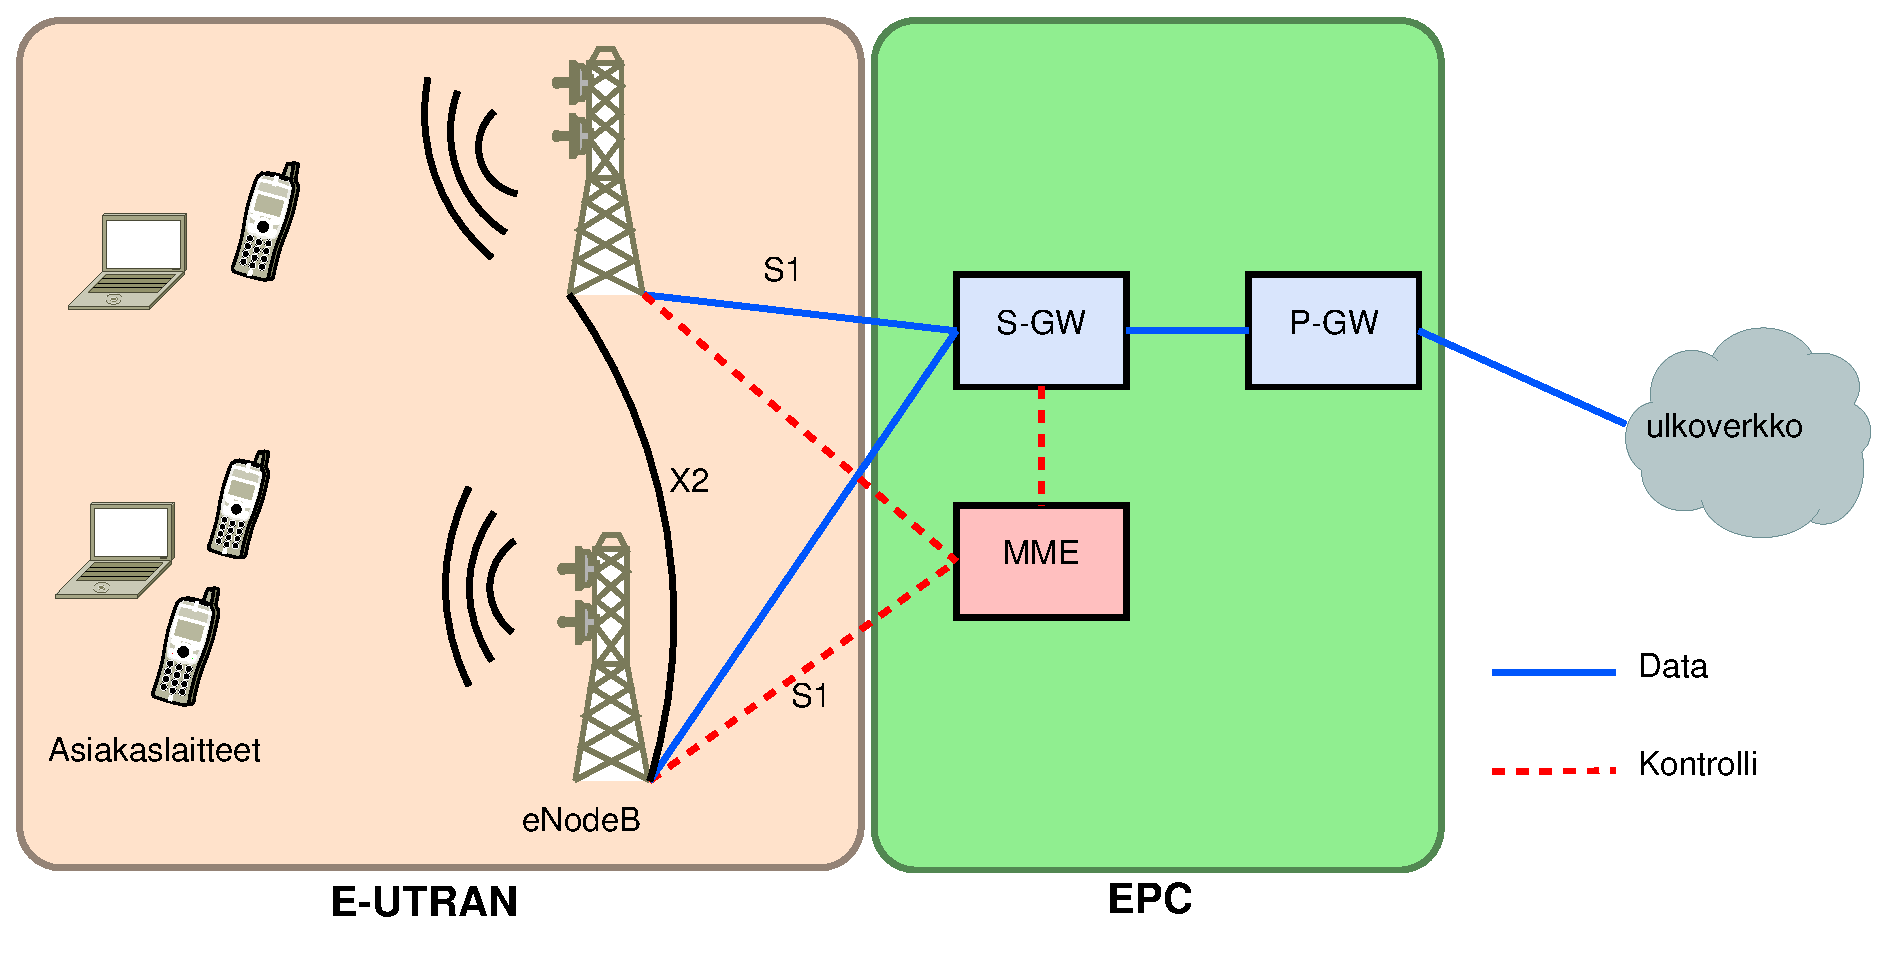
\includegraphics[width = \textwidth]{EPC.eps}
\caption{Yksinkertaistettu LTE-tyyppisen mobiiliverkon rakenne.} \label{fig:mobiarch}
\end{figure}

Tässä tutkielmassa käsiteltävät reuna-arkkitehtuurit sisältävät yhdistävänä tekijänä tavoitteen toimia mobiiliverkon yhteydessä. 
Täten reuna-arkkitehtuurien suunnittelupäätöksiä tarkasteltaessa on tarpeen ymmärtää mobiiliverkon osat yleisellä tasolla.
Yksinkertaisuuden vuoksi tämän tutkielman puitteissa mobiiliverkoksi oletetaan LTE:n mukainen arkkitehtuuri, joka koostuu E-UTRAN tyyppisestä radioverkosta ja EPC tyyppisestä runkoverkosta.
Seuraavaksi käydään läpi mobiiliverkon arkkitehtuurin tämän tutkielman kannalta merkitykselliset toimijat ja toiminnot.

Korkealla tasolla tarkasteltuna mobiiliverkko koostuu kahdesta osiosta: radioverkosta ja runkoverkosta. 3GPP kehittämässä LTE (Long Term Evolution) standardissa radioverkon sisältävä osuus on nimeltään E-UTRAN (Evolved UMTS Terrestrial Radio Access Network) ja runkoverkon osuus on nimeltään EPC (Evolved Packet Core).
E-UTRAN ja EPC väliset yhteydet on kuvattu kuvassa \ref{fig:mobiarch}.

E-UTRAN tehtävänä on toimia rajapintana asiakaslaitteen ja EPC:n välillä. 
E-UTRAN sisältää verkon puolella pääasiallisena toimijana eNodeB (Evolved nodeB) tyyppisiä tukiasemia \cite{etsieutran}.
Tukiasemista on olemassa muutamia erilaisia variaatioita, mutta tässä tutkielmassa käsitellään ainoastaan perustapausta.
Tukiasema on asiakaslaitetta lähimpänä sijaitseva funktionaalinen verkon osa ja sen seurauksena se on houkutteleva kohde reunalaskennan ratkaisuille. Tietoliikenteen näkökulmasta tukiaseman voi ajatella \textit{reunan} viimeisenä etappina ennen asiakaslaitteita. 

ENodeB tarjoaa asiakaslaitteiden suuntaan radioyhteyden.
EPC:n suuntaan eNodeB:t ovat yhteydessä S1 rajapinnan avulla.
Lisäksi eNodeB:t voivat olla toisiinsa yhteydessä X2 rajapinnan kautta.
S1:stä käytetään eNodeB:n ja EPC:n väliseen kommunikointiin. Tämä sisältää sekä hallinnollisen viestinnän, että asiakkaan tietoliikenteen kuljettamisen.
X2 rajapintaa puolestaan käytetään tukiasemien väliseen kommunikointiin. 
ENodeB välisten X2 yhteyksien tavoitteena on nopeuttaa tukiasemien välistä kommunikaatiota, esimerkiksi handoverin yhteydessä tehtävää asiakaskontekstin siirtoa varten \cite{3gpplte}.
Handoverilla tarkoitetaan asiakaslaitteen radioyhteyden siirtoa toiselle tukiasemalle. Handover käsitellään tarkemmin kappaleessa \ref{livemigraatio}.

Mobiiliverkon runkona toimiva EPC koostuu useista loogisista komponenteista.
Tämä siis tarkoittaa että toiminnallisuudet voivat fyysisesti sijaita samassa laitteessa. 
Tässä tutkielmassa on tarpeen ymmärtää perusteet seuraavista alikomponentista: MME (Mobility Management Entity), S-GW (Serving Gateway) ja PDN GW (P-GW, Packet data network gateway) \cite{etsilte}.
\begin{itemize}
\item \textbf{MME} on EPC:n hallinnollinen entiteetti joka vastaa muun muassa asiakaslaitteen tunnistamisesta ja handoveriin liittyvistä toimista EPC:n sisällä. Toisin kuin S-GW ja P-GW, MME ei käsittele asiakaslaitteiden tietoliikennettä.
\item \textbf{S-GW} eli palveluyhdyskäytävä toimii asiakaslaitteen EPC:n sisäisenä kiintopisteenä.  S-GW reitittää asiakaslaitteen liikennettä P-GW:n ja E-UTRAN välillä.
\item \textbf{P-GW} eli pakettiverkon yhdyskäytävän tehtävänä on toimia asiakaslaitteen ja mobiiliverkon ulkopuolisten IP-verkkojen yhteyspisteenä.
\end{itemize}
\cite{3gppepc}

Mobiiliverkossa käytävä kommunikaatio voidaan jakaa kahteen kerrokseen: kontrollikerrokseen ja tietoliikennekerrokseen.
Kontrollikerroksella välitettävät viestit ovat tarkoitettu hallinnollisiin toimintoihin mobiiliverkon sisällä. 
Tietoliikennekerros välittää asiakkaan tietoliikennettä internetin ja asiakaslaitteen välillä.
Asiakkaan tietoliikenne kulkee tukiaseman ja P-GW:n välillä GTP-tunneloituna (GPRS Tunnelling Protocol) \cite{puente15seamless}. Tämä tarkoittaa että mobiiliverkon sisällä tietoliikennettä ei ohjata asiakaslaitteen tietoliikenteen tunnisteiden pohjalta. 


\subsection{Reuna-arkkitehtuuri}
%Määrittele mikä on reuna-arkkitehtuuri


Tässä tutkielmassa käsiteltävät arkkitehtuurit ovat pääasiassa tyypiltään oletusarkkitehtuureja (framework). 
Tämänkaltaisen arkkitehturin tarkoituksena on jakaa järjestelmä toiminnallisiin osiin fyysisellä ja ohjelmallisella tasolla \cite{ohark}. Se siis kuvaa järjestelmän rakenneosien tehtävät.
Oletusarkkitehtuuria voidaan hyödyntää varsinaista toteutettavaa järjestelmää suunniteltaessa.

Kappaleessa \ref{reunatoimijat} kuvattujen reunan toimijoiden osalta reuna-arkkitehtuurit keskittyvät kuvaamaan reunasolmun ja reuna-alustan tehtäviä. Lisäksi reuna-arkkitehtuurit kuvaavat koko järjestelmän osana toista järjestelmää, jolloin reunajärjestelmä itsessään on komponentti suuremmassa järjestelmässä. Tällä tasolla tarkasteltu arkkitehtuuri jättää avoimeksi reunasovelluksien toiminnan ja keskittyy kuvaamaan reunasovelluksien sijaintia järjestelmässä.

Tämän tutkielman puitteissa arkkitehtuurilla tarkoitetaan reuna-alustan ja reunasolmujen muodostamaa järjestelmää. Reuna-alustan toiminnallisuuksia voisi eritellä vielä tarkemmin, etenkin reunasovelluksien hallinnan osalta. Cloudlet on konkreettinen toteutus reuna-alustan reunasovelluksia hallinnoivasta osasta, mutta se ei kata kuin yhden reunasolmun kerrallaan. 
Tämän lisäksi olemassa on reunasolmujen välisestä hallinnasta vastaava kerros, tosin tämä kerros voi olla ulkoistettu erillisille hallinnolliselle toimijalle, jolloin hallinnollinen osa reuna-alustasta on varsinaisten reunasolmujen ulkopuolella. 

Reunasovelluksien toimintaa ei käsitellä tarkemmin. Taxonomy paperissa on hyvä jaottelu erilaisista sovelluksista. Tämä aihepiiri laajenee sovelluksien jakamiseen osittain reunalla suoritettaviin (offloading) tai mobiilisovelluksen suoritusta tukeviin sovelluksiin. 

